\documentclass[12pt, letterpaper]{article}
\usepackage{hyperref}
\usepackage{setspace}
\usepackage[table]{xcolor}
\usepackage{graphicx}
\usepackage{booktabs}
\usepackage{float}
\usepackage{subfig}
\title{Predicting heart failure patient survivability}
\author{Matthew Devaney}
\date{August 1, 2025}

\begin{document}
	\maketitle
	\onehalfspacing
	\section*{Abstract}
	
	Heart failure is an increasingly common and potentially fatal condition that occurs when a person's heart is unable to pump or fill with enough blood to support the body. In this study, I examined a data set of 300 heart failure patients and their associated lifestyle and biological data. The purpose of this study is to 1: determine the biomarkers with the strongest predictive power and 2: create a robust predictive model to determine patient survivability. First, I performed an exploratory data analysis of the patient data. Using these insights, I trained several classifiers to determine survivability. Through this process, I find ejection fraction and serum creatinine are the 2 most effective predictors of a heart failure patient's survival. 
	
	\section{Introduction}
	
	Heart failure, also known as congestive heart failure (CHF), is a condition that occurs when a person's heart is unable to either pump or fill with enough blood to support his or her bodily function. People with heart failure often experience shortness of breath, excess fatigue, and swelling among other symptoms. It is an increasingly common health problem and the leading cause of hospitalizations in older adults. Between 2017-2020, 6.7 million Americans over the age of 20 had heart failure, a number expected to rise to over 8 million in 2030 \cite{hf_info}. In 2022, CHF was mentioned on 457,212 death certificates and responsible for 13.9\% of all causes of death in the United States \cite{cdcAboutHeart}. One study found that patients had a ten-year survival rate of 27\% (compared to 75\% in the general population) - similar to certain cancers \cite{nihChronicHeart}. The economic impact is also significant, with costs related to CHF projected to rise from \$30.7 billion in 2012 to \$69.8 billion by 2030 \cite{hf_info}.
	
	The goal of this study is to examine several biomarkers and their associations with CHF patient survival outcomes. In particular, the patient data come from the Faisalabad Institute of Cardiology and the Allied Hospital in Faisalabad in Punjab, Pakistan. They were recorded for a period of time between April-December 2015. All patients had left ventricular systolic dysfunction and previous heart failures.
	
	I will examine the data and visualize relationships found between the target variable (patient survival) and the predictors. After finding the most important predictors, I will create classifiers to predict a patient's survival and evaluate their performance.

	\section{Data}
	
	There are 6 binary variables: death event, anaemia, diabetes, high blood pressure, sex, and smoking. The death event was recorded as whether the patient died during the follow-up time. anaemia occurs when the body does not have enough red blood cells to transport oxygen to tissue and is a common comorbidity of heart failure \cite{doi:10.1161/CIRCULATIONAHA.118.030099}. Diabetes affects how the body uses sugar. One study found patients with diabetes mellitus have two times the risk of developing heart failure \cite{doi:10.1161/CIRCRESAHA.118.311371}. High blood pressure occurs when the force of blood pushing against the artery walls is too high. This can lead to growth of the left ventricle, which can progress to heart failure \cite{hbp}.
	
	The other 7 continuous variables are age, creatinine phosphokinase, ejection fraction, platelets, serum creatinine, serum sodium, and follow up time. Elevated levels of CPK in the blood can indicate muscle tissue damage, such as rhabdomyolosis and acute myocardial infarction \cite{cpkArticle}. The ejection fraction models the percentage of blood pumped out of the left ventricle per contraction. Fractions less than 40\% indicate possible heart failure \cite{ejectionFraction} Abnormal platelet levels can affect the blood's ability to clot and repair blood cells. Too many platelets can lead to heart attack or stroke. Too few platelets can cause frequent bleeding \cite{platelets}. Abnormal serum creatinine levels can indicate poor kidney function, which can affect heart function \cite{creatinine}. Lastly, low sodium levels have also been shown to occur alongside heart failure \cite{sodium}.
	
	\begin{figure}[H]
		\centering
		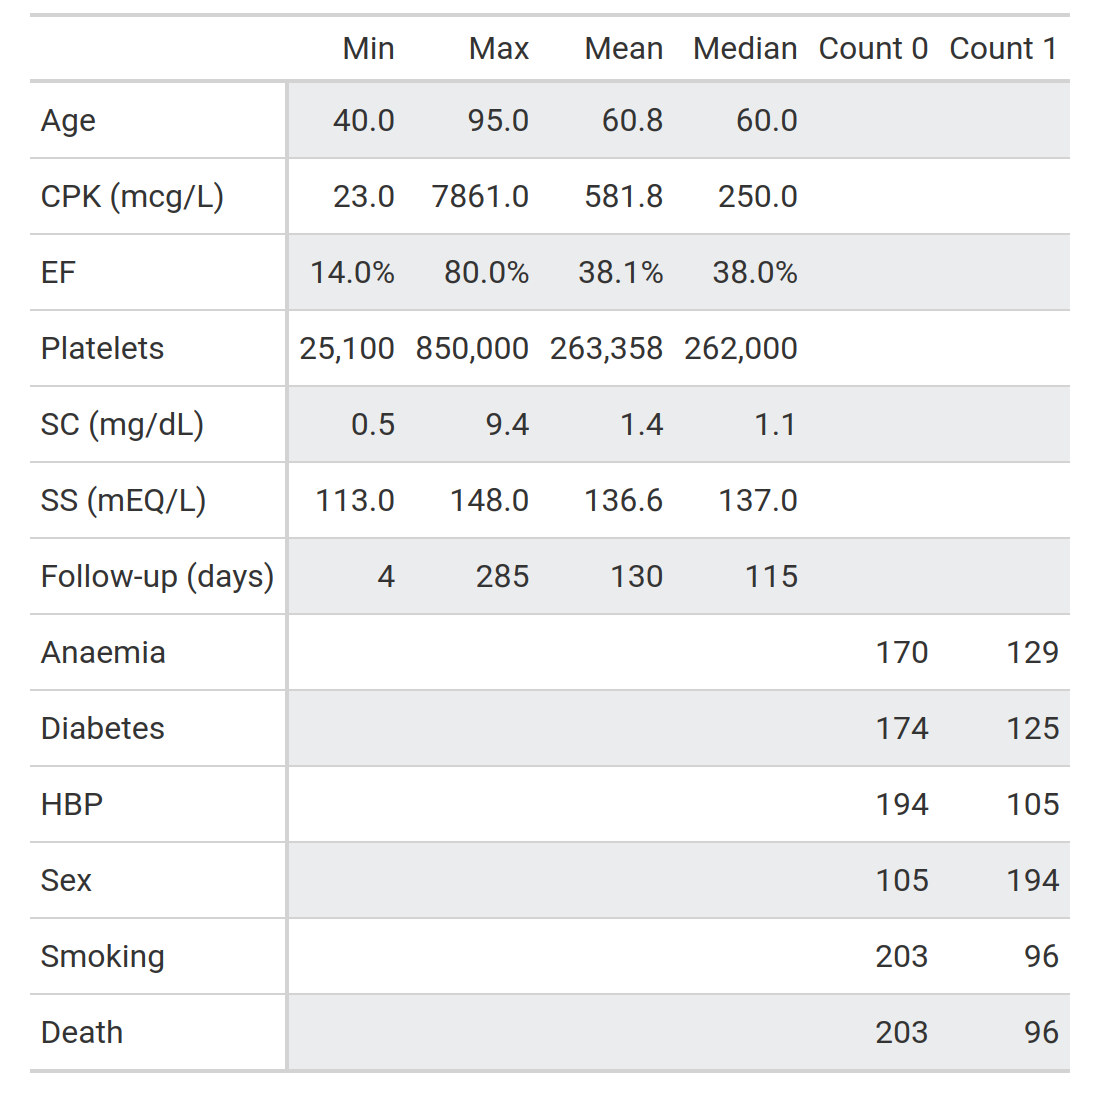
\includegraphics[width=0.70\linewidth]{figs/variable_stats.png}
		\caption{Summary statistics of the data}
		\label{fig:sum_stats}
	\end{figure}

	
	The percentage of deaths per age group shows a steady increase as patient age increases. \textasciitilde36\% of patients aged 61 to 90 died and accounted for 50\% of all deaths in the data set. The number of deaths is equally distributed between male and female patients, suggesting there is no difference between the two groups. Furthermore, the majority of deaths occur within the first 2 months of follow-up time, with a spike of patients dying between the 5th and 6th month. \textasciitilde85\% of patients who had a follow-up within the first 2 months died and \textasciitilde56\% of all deaths were accounted for by these patients. It is possible that the follow-up time is a function of the patient's condition, such that the most sickly patients have shorter follow-up times. Lastly, each of the health conditions provided in the data set have a similar death rate. (Note: patients with multiple conditions were included in each measurement e.g. a patient with anaemia and diabetes was counted once for anaemia and again for diabetes).
	
	\begin{figure}[H]
		\centering
		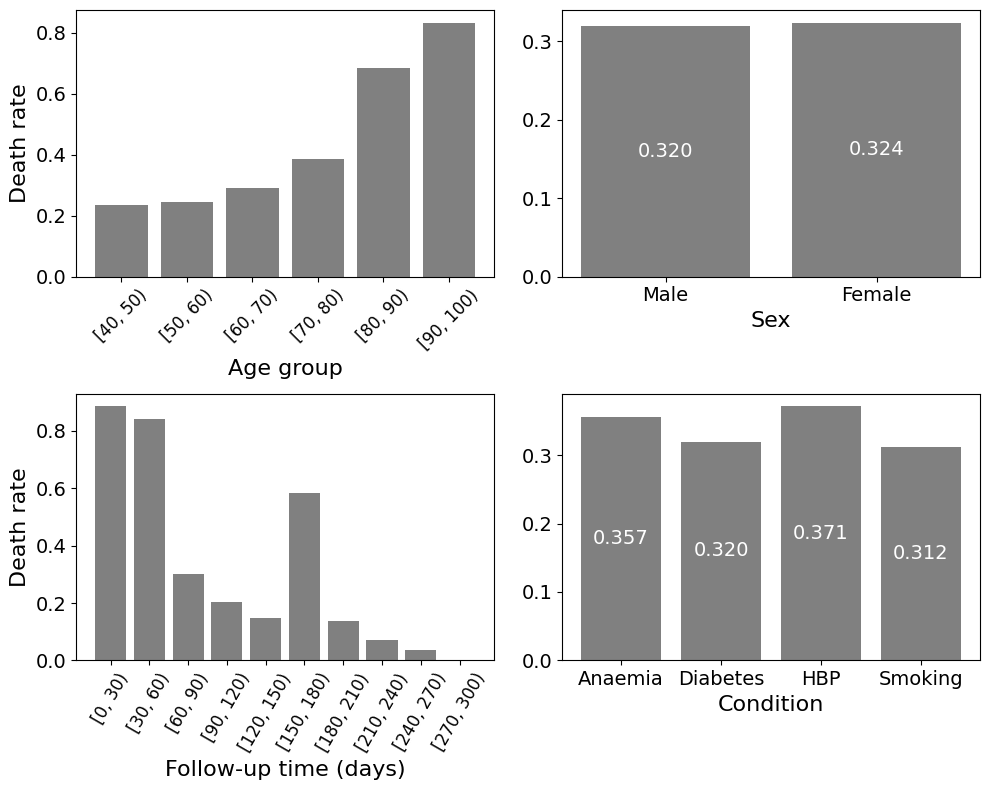
\includegraphics[width=0.70\linewidth]{figs/death_rates.png}
		\caption{Top left: death rate per 10 year age group. Top right: death rate per sex. Bottom left: death rate per follow-up period. Bottom right: death rate of patients with each condition.}
		\label{fig:death_rates}
	\end{figure}
	
	The last part of the data I will explore is the correlation between features. From the correlation matrix, we can see that age, anaemia, serum creatinine (SC), and follow-up time have the strongest correlations with death. This indicates that there is at least some relation between the features and patient survival.
	
	\begin{figure}[H]
		\centering
		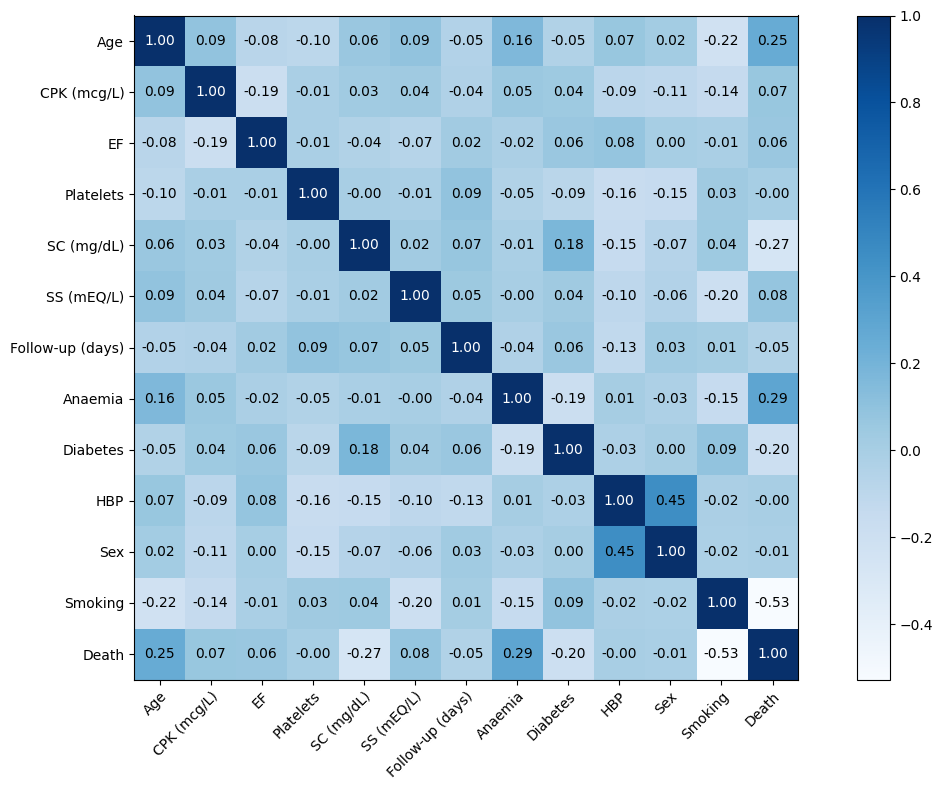
\includegraphics[width=0.8\linewidth]{figs/corr_mat.png}
		\caption{Correlation matrix showing the pairwise correlations between all 13 features. Darker colors indicate a strong positive correlation, while lighter colors indicate a strong negative correlation.}
		\label{fig:corr_mat}
	\end{figure}
	
	
	\section{Analysis}
	Now that I have have explored the data set, I will create models to predict the survival outcome of a heart failure patient. After, I will compare them to choose a final model to fine tune. First, I will address the scale of the data. Features like 'platelets' and 'serum creatinine' are on vastly different scales. To alleviate this, I will standardize all of the continuous features. Also, I have chosen to omit the 'follow-up time' feature to focus on features that could be measured immediately.
	
	I will start by fitting the following machine learning models: logistic regression, support vector machine (with RBF kernel), random forest (500 trees), and XGBoost (1000 trees) using all remaining features. I will assess the model performance with 10-fold cross validation using recall as a scoring metric. Recall is used to emphasize the importance of detecting all positive examples of heart failure. I will also use the following scoring metrics on the test data set: accuracy, precision, F1, ROC AUC, and Matthews' correlation coefficient (MCC). Lastly, to deal with the imbalanced classes (96 deaths vs 203 survivals), I employ the 'balanced' feature of scikit-learn's estimators to penalize wrong predictions on the minority class.
	
	\begin{figure}[H]
		\centering
		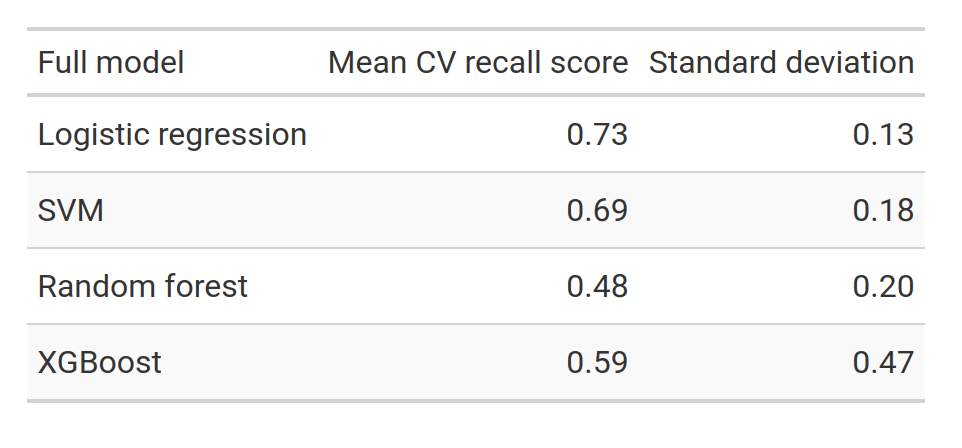
\includegraphics[width=0.8\linewidth]{figs/full_model.png}
		\caption{10-fold CV results of models fitted with all features.}
		\label{fig:full_model}
	\end{figure}
	
	As you can see, logistic regression with a balanced class penalty performed the best, while the random forest with 500 decision trees was the weakest. Before I proceed with changing the models, let's examine the learning curves for each of the 4 models. Unfortunately, using the full feature set results in overfitting. In particular, the random forest and XGBoost models have a large gap between training and test performance, which could be due to poor hyperparameter choice.
	
	\begin{figure}[H]
		\centering
		\begin{tabular}{cccc}
			\subfloat[Logistic Regression]{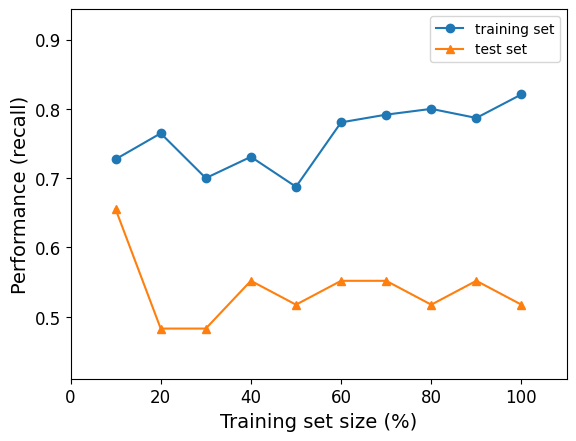
\includegraphics[width = 2.5in]{figs/lr.png}} &
			\subfloat[SVM]{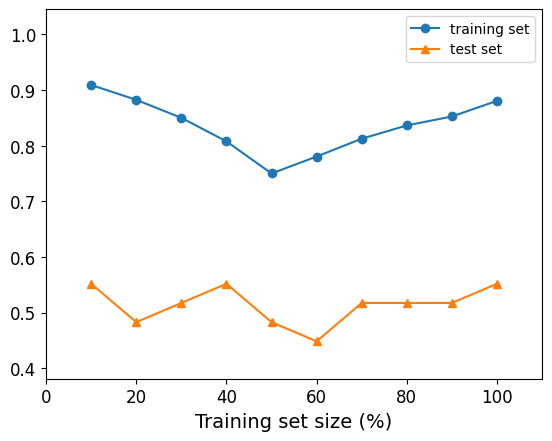
\includegraphics[width = 2.5in]{figs/svm.png}} \\
			\subfloat[Random forest]{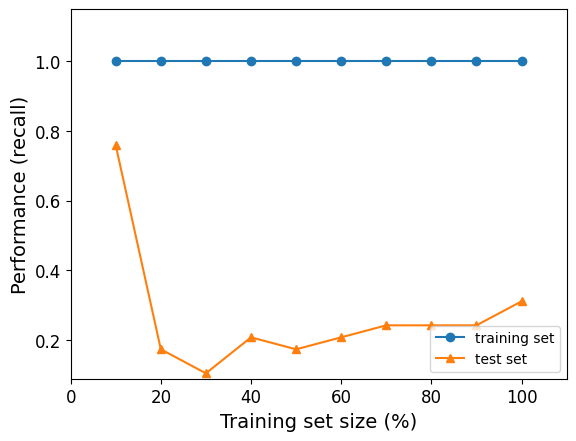
\includegraphics[width = 2.5in]{figs/rf.png}} &
			\subfloat[XGBoost]{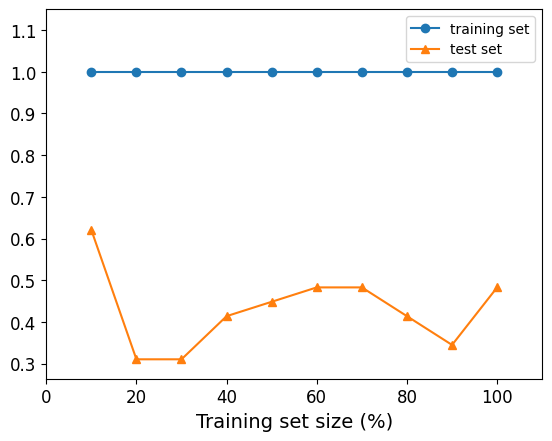
\includegraphics[width = 2.5in]{figs/gb.png}}
		\end{tabular}
		\caption{Learning curves of the 4 classifiers}
	\end{figure}
	
	To alleviate the overfitting, I will use a random forest to assess feature importance and perform feature selection to shrink the number of model parameters. From the figure, it is clear that serum creatinine and ejection fraction are the two most important features in the data set. Now, I will train the models again, this time using just serum creatinine and ejection fraction as the feature input.
	
	\begin{figure}[H]
		\centering
		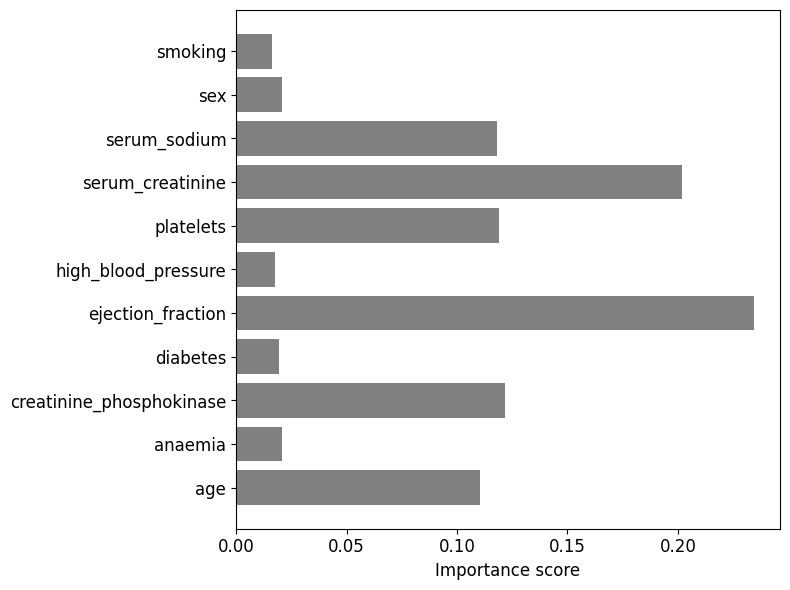
\includegraphics[width=0.8\linewidth]{figs/feat_imp.png}
		\caption{Feature importance ranking from a random forest with 500 trees.}
		\label{fig:feat_imp}
	\end{figure}
	
	Based on the cross validation performance and the learning curves, all 4 classifiers improved when using just 2 features as opposed to the entire feature set. Using less features likely reduced the variance of the models, which explains the smaller gap between the training and testing curves.
		
	\begin{figure}[H]
		\centering
		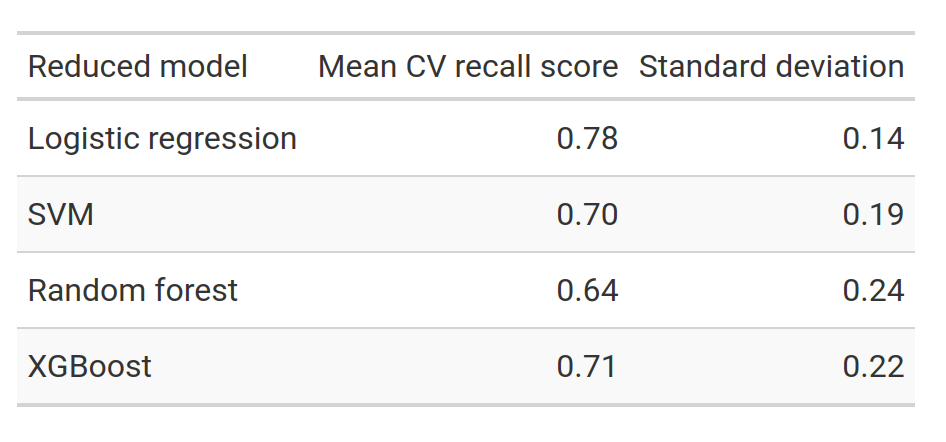
\includegraphics[width=0.8\linewidth]{figs/red_cv.png}
		\caption{10-fold CV results models fitted with reduced features}
		\label{fig:red_cv}
	\end{figure}
	
	\begin{figure}[H]
		\centering
		\begin{tabular}{cccc}
			\subfloat[Logistic Regression]{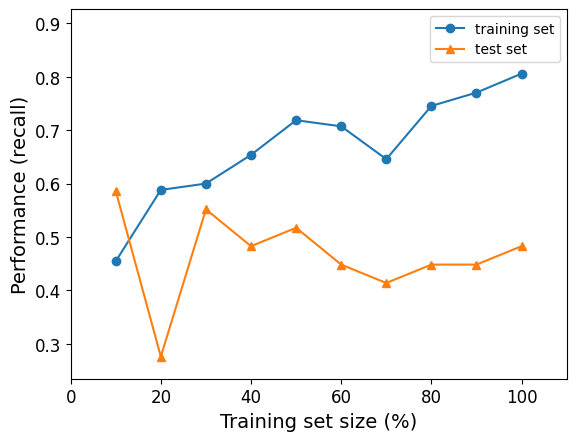
\includegraphics[width = 2.5in]{figs/lr_red.png}} &
			\subfloat[SVM]{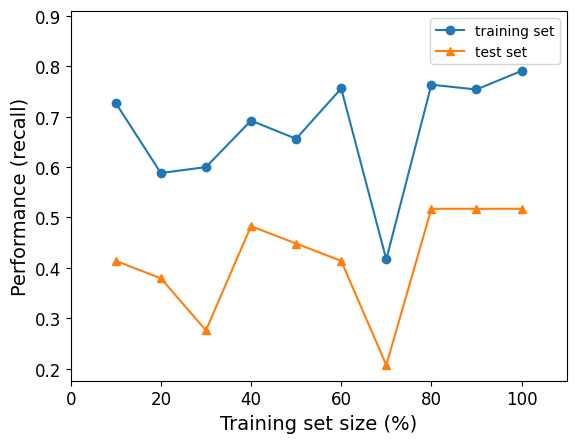
\includegraphics[width = 2.5in]{figs/svm_red.png}} \\
			\subfloat[Random forest]{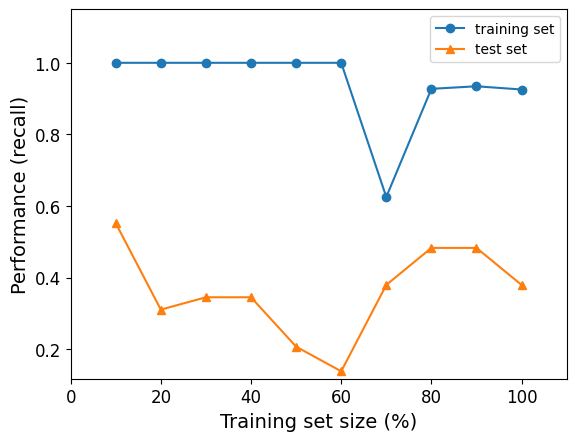
\includegraphics[width = 2.5in]{figs/rf_red.png}} &
			\subfloat[XGBoost]{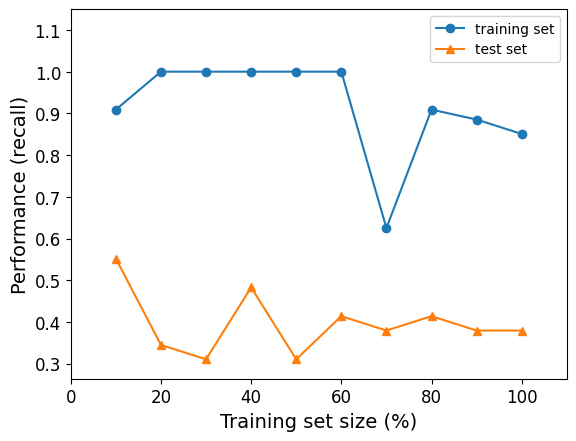
\includegraphics[width = 2.5in]{figs/gb_red.png}}
		\end{tabular}
		\caption{Learning curves of the 4 reduced classifiers}
	\end{figure}
	
	The tree-based methods are still suffering from high variance, so I will implement a grid search to find better hyperparameter values. The best random forest model contained the following parameters: 'max\_depth': None, 'min\_samples\_leaf': 4, 'min\_samples\_split': 2, and 'n\_estimators': 200. Furthermore, the best XGBoost model contained the following parameters: 'colsample\_bytree': 0.7, 'gamma': 0, 'learning\_rate': 0.01, 'max\_depth': None, 'min\_child\_weight': 2, 'n\_estimators': 200, and 'subsample': 0.7. This improved both classifiers greatly, with each achieving a cross validation score of 0.78 and 0.81, respectively.
	
	The final performance test was performed with the remaining 30\% of the data set not used for training. Overall, the models performed similarly well, with the SVM and XGBoost models performing slightly better than the logistic regression and random forest model. It is important to keep in mind that these results come from just two predictors.
	
	\begin{figure}[H]
		\centering
		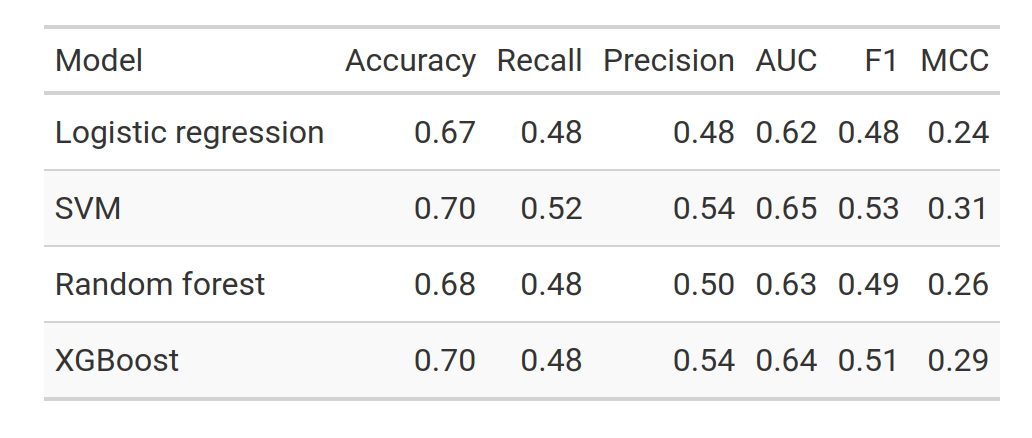
\includegraphics[width=0.9\linewidth]{figs/final_test.png}
		\caption{Various scoring metrics based on the test data set}
		\label{fig:final_test}
	\end{figure}
	
	\section{Conclusion}
	
	The goal of this study was to predict heart failure patient survival. Through exploratory data analysis, I found that the risk of death increased as the patient's age increased. Conversely, the risk of death decreased as follow-up time increased. I found that male and female patients had the same death rate. The health conditions included in the data (high blood pressure, anaemia, diabetes, and smoking) followed a similar trend, with only small differences in death rate between patients with each condition. Then, I created a correlation matrix and found that age, anaemia, serum creatinine (SC), and follow-up time were most strongly correlated with patient survival outcome.
	
	After finding some influential predictors, I created 4 classifiers (logistic regression, SVM, random forest, XGBoost), using the full feature set. After evaluating the cross validation results, I used a random forest model to assess variable importance in hopes to reduce overfitting. I refit the models using just the two most important features, which reduced the degree of overfitting. Since the tree-based methods were still overfitting, I implemented a grid search to find the best hyperparameters for these two methods. Finally, I used the test dataset to evaluate the performance of the tuned classifiers.
	
	The best performing models were the SVM and XGBoost model, according to Figure \ref{fig:final_test}. The random forest and logistic regression were not far behind in terms of performance, though. For using just 2 predictors, the performance of the models is quite impressive.
	
	Through exploring and modeling the data, I came to the conclusion that the 2 most important predictors of a heart failure patient's survival are ejection fraction and serum creatinine. Ejection fraction models the heart's blood flow, which is obstructed in a heart failure patient. Muscle damage can increase serum creatinine levels, so higher levels may also indicate heart failure. The classifier I built demonstrate their predictive power. These variables should be examined thoroughly in a patient who has heart failure. Careful monitoring of these variables may be able to predict who needs care most urgently.
	
	\subsection{Limitations and further analysis}
	
	This data set featured imbalanced classes, with about one-third of patients dying and the other two-thirds of patients surviving. It would be beneficial to have a larger sample size and more balanced classes. If balanced classes could not be obtained, then resampling techniques or synthetic methods such as SMOTE could be applied. Moreover, additional predictors would be beneficial such as a person's height and weight. For further analysis, one could produce modeling involving the follow-up time as a variable, as it was shown to be highly correlated with the death event.
	
\nocite{*}
\bibliographystyle{apalike}	
\bibliography{bibliography.bib}
\end{document}